\chapter{Appendix B: Cost Models}
\label{app:b}

\section{Static NPV Model}
The static model described in Section \ref{ch4:cm_concept} was implemented in Microsoft Excel as a single sheet for cost analysis. Figures \ref{fig:static_model_sheet1}-\ref{fig:static_model_sheet2} show the model when flow rate is pre-defined and capacity depends on the input temperature of the produced brine. Not shown is the supporting look-up table for the EIA STEO-based electricity price forecast (Figure \ref{fig:electricity_pricing}).

\begin{figure}[!htp]
\centering
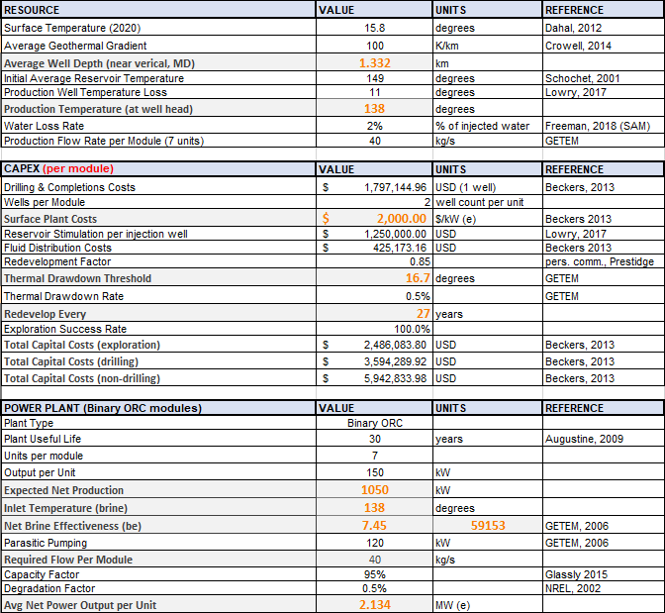
\includegraphics[width=\textwidth]{templates/images/Figure-Static_Model_SheetA.png}
\caption[Static cost model worksheet (part 1)]{First part of geothermal power plant expansion static NPV cost model.}
\label{fig:static_model_sheet1}
\end{figure}

\begin{figure}[!htp]
\centering
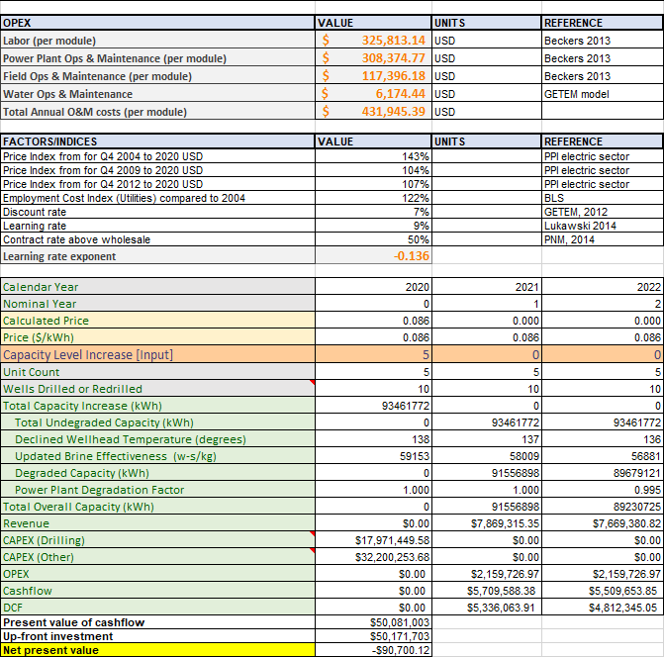
\includegraphics[width=\textwidth]{templates/images/Figure-Static_Model_SheetB.png}
\caption[Static cost model worksheet (part 2)]{Second part of geothermal power plant expansion static NPV cost model. The yearly breakdown of cost and revenue only extends out to year 2 for visualization purposes but continues to year 30 in the actual spreadsheet.}
\label{fig:static_model_sheet2}
\end{figure}

\section{Flexible NPV Models}

\subsection{Redevelop Only Case Model}

\subsection{Redevelop and Grow Case Model}

\subsection{Full Flexibility Case Model}